\documentclass{standalone}
\usepackage{tikz}
\usepackage{ctex,siunitx}
\setCJKmainfont{Noto Serif CJK SC}
\usepackage{tkz-euclide}
\usepackage{amsmath}
\usetikzlibrary{patterns, calc,3d}
\usetikzlibrary {decorations.pathmorphing,decorations.pathreplacing,decorations.shapes}
\begin{document}
\small
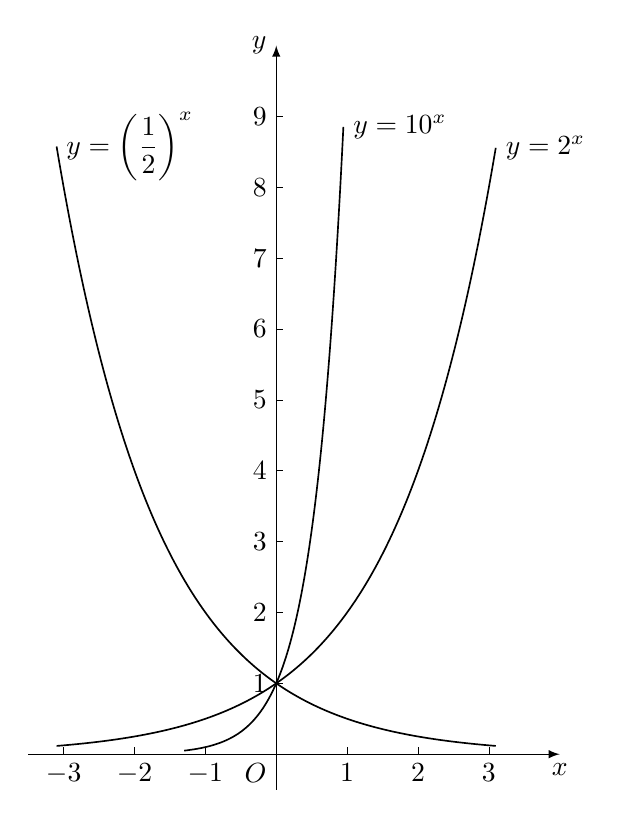
\begin{tikzpicture}[>=latex,scale=0.9]
  \draw[->](-3.5,0)--(4,0)node[below]{$x$};
  \draw[->](0,-0.5)--(0,10)node[left]{$y$};
  \node at (0,0)[below left]{$O$};
  \foreach \x in {1,...,3} 
    {
      \draw[very thin](\x,0)node[below]{$\x$}--++(0,0.1);
      \draw[very thin](-\x,0)node[below]{$-\x$}--++(0,0.1);
    }
  \foreach \x in {1,...,9} 
    {
      \draw[very thin](0,\x)node[left]{$\x$}--++(0.1,0);
    }
  \draw[semithick,samples=200,domain=-3.1:3.1]plot(\x,{pow(2.0,\x)})node[right]{$y=2^x$};
  \draw[semithick,samples=200,domain=-1.3:0.95]plot(\x,{pow(10,\x)})node[right]{$y=10^x$};
  \draw[semithick,samples=200,domain=-3.1:3.1]plot(\x,{pow(0.5,\x)});
  \node at (-3.1,{pow(0.5,-3.1)})[right]{$y=\left(\dfrac12\right)^x$};
\end{tikzpicture}
\end{document}